\section{Obiettivi di qualità} 
\subsection{Qualità di processo}

Al fine di garantire la qualità del prodotto in ogni fase di realizzazione, si deve garantire la qualità dei processi che lo definiscono; per questo motivo si è deciso di utilizzare lo standard ISO/IEC 15504 denominato SPICE, che rende disponibili strumenti adatti a valutarli.

\subsection{Qualità di prodotto}
Per garantire la qualità del prodotto, si è deciso di seguire le indicazioni fornite dallo
standard ISO/IEC 9126:2001 sostituito dal successivo ISO/IEC 25010:2011. Questo
documento fornisce un modello per valutare la qualità esterna, cioè nell’ambiente
di utilizzo, ed interna, cioè indipendente dall’ambiente, di un software individuando
sei caratteristiche principali atte a rendere il prodotto qualitativamente accettabile.

\begin{figure}[h]
  \centering
    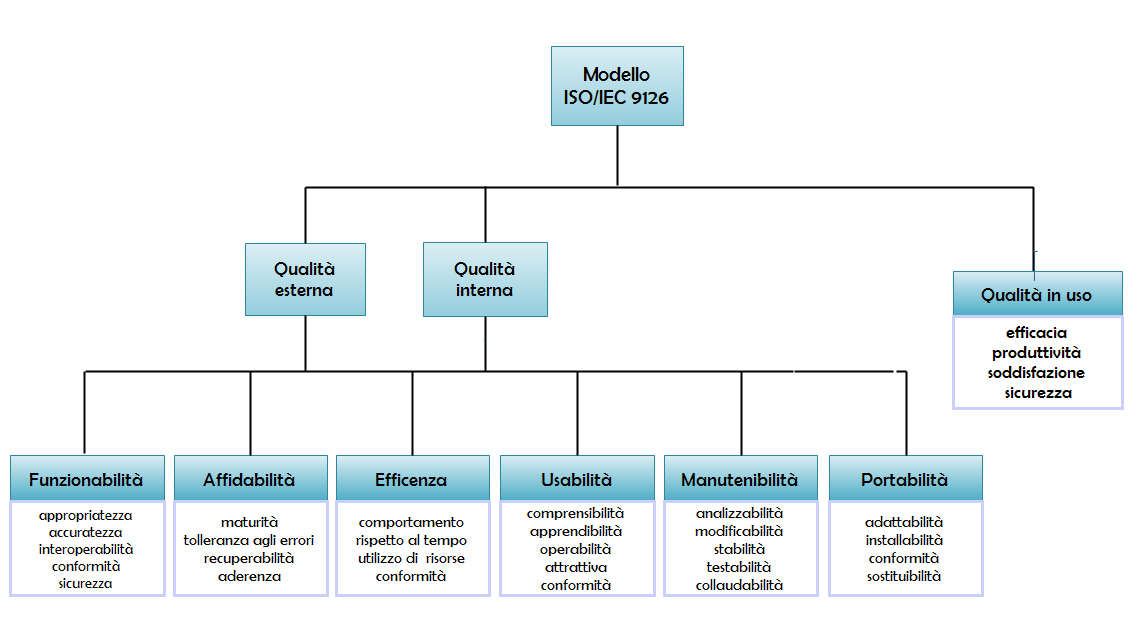
\includegraphics[width=0.5\textwidth]{./images/ISO-IEC_9126}
  \caption{Rappresentazione del modello ISO/IEC 9126:2001}
  \label{fig:ISO-IEC_9126}
\end{figure}


\subsubsection{Funzionalità}
E' un requisito funzionale che indica la capacità del software di soddisfare le esigenze esposte dal capitolato ed individuate durante l’analisi dei requisiti, per valutare questa caratteristica si considerano l' appropriatezza e l' accuratezza delle funzioni offerte, l'interoperabilità del prodotto rispetto ai diversi sistemi e la sicurezza offerta per la protezione dei dati.\\ 
Si sarà ottenuto un buon risultato in questo settore quando il software avrà superato in maniera positiva tutti i test e assicurerà copertura a tutti
i requisiti obbligatori.

\subsubsection{Affidabilità}

E' un requisito non funzionale che indica la capacità del software di svolgere correttamente il suo compito, mantenendo delle buone prestazioni anche al variare dell' ambiente nel tempo, per questo vengono considerate la sua tolleranza agli errori, la capacità di evitare fallimenti nell’esecuzione a seguito di malfunzionamenti,
detta maturità, e la recuperabilità dei dati e delle prestazioni nell' eventualità di un malfunzionamento inevitabile. Il prodotto può considerarsi affidabile se il numero di esecuzioni andate a buon fine è sufficientemente grande rispetto al numero di esecuzioni totali.

\subsubsection{Efficienza}

E'un requisito non funzionale che indica il rapporto tra le prestazioni e le risorse disponibili, si valuta cioè se il software utilizza al meglio le risorse a sua disposizione per fornire le funzionalità richieste, considerando il suo comportamento rispetto al tempo, ossia la velocità di risposta e di elaborazione in determinate condizioni, e rispetto all’uso delle risorse, ossia la sua capacità di utilizzare la quantità adeguata di risorse per eseguire le funzioni richieste. Un modo per valutare l’efficienza di un software è calcolarne i tempi di attesa in seguito all’esecuzione di un comando, tuttavia, nel caso del prodotto Premi, l' efficienza è limitata anche dallo stato della rete e dall' utilizzo di componenti grafiche quali video o immagini , per questo motivo il gruppo non può garantire tempi di risposta brevi per ogni azione compiuta dall’utente, ma si impegnerà a non appesantire ulteriormente tali componenti.

\subsubsection{Usabilità}

E' un requisito non funzionale che indica la capacità del software di essere compreso,appreso ed usato con soddisfazione dall' utente, per far ciò il prodotto deve soddisfare condizioni di comprensibilità, apprendibilità ed operabilità, deve inoltre avere una certa attrattiva nei confronti dell 'utente allo scopo di rendergliene piacevole l’utilizzo. Questa caratteristica non è facilmente misurabile in quanto non esistono metriche per quantificarla, perciò si farà affidamento alle linee guida del material design fornite dalla Google dato l'alto tasso di penetrazione che hanno avuto nel mercato rispetto ad altre linee guida.

\subsubsection{Manutenibilità}
E' un requisito non funzionale che indica la capacità del software di essere corretto,migliorato o adattato con un impegno contenuto, a tale scopo esso deve essere facilmente analizzabile e modificabile, deve garantire stabilità a seguito di modifiche e testabilità di tali modifiche. Per misurare questa caratteristica esistono una serie di metriche descritte nella sezione ----> Metriche e quantificabili 

\subsubsection{Portabilità}

E' un requisito non funzionale che indica la capacità del software di adattarsi al cambio di dispositivo e sistema operativo ,limitando la necessità di apportare cambiamenti.\\
Per soddisfare questa caratteristica, come espresso dal capitolato, è necessario che il software funzioni sia su computer (indipendentemente dal loro sistema operativo) e su dispositivi mobile Android,IOs e Windows Phone.

\subsection{Procedure di controllo di qualità di processo}
Per applicare il modello SPICE si utilizzerà il ciclo di Deming. Il ciclo di Deming è un sistema iterativo per il miglioramento continuo della qualità
dei processi e dei prodotti da essi risultanti che permette di riconoscere lo stato di avanzamento di un progetto fornendo un metodo di lavoro logico e sistematico.

\begin{figure}[h]
  \centering
    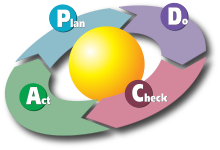
\includegraphics[width=0.5\textwidth]{./images/deming}
  \caption{Schema PDCA}
  \label{fig:deming}
\end{figure}

 E' chiamato anche ciclo PDCA, in quanto è definito dall'iterazione delle quattro fasi:
 
\begin{itemize}
\item 
\textbf{Plan}:
si stabiliscono gli obiettivi e i processi necessari a ottenere risultati conformi agli obiettivi attesi;
\item 
\textbf{Do}:
si implementa il piano, si esegue il processo e si realizza il prodotto. Si raccolgono dati da analizzare nei passi successivi;
\item
\textbf{Check}:
si studiano i risultati ottenuti tramite la raccolta dei dati nella fase "Do" e si paragonano con i risultati attesi (gli obiettivi stabiliti nella fase "Plan"), per verificare la presenza di incongruenze. Si evidenziano le divergenze di implementazione rispetto al piano;
\item 
\textbf{Act}:
se la fase di Check evidenzia che gli obiettivi fissati nel Plan e implementati sul Do rappresentano un miglioramento rispetto alla baseline precedente, si stabilisce una nuova baseline. In caso contrario la baseline resta la precedente. In enrambi i casi se la fase di Check ha evidenziato differenze rispetto alle aspettative, sarà necessario svolgere nuovamente il ciclo di PDCA.
\end{itemize}